\chapter{SYSTEM DESIGN AND ARCHITECTURE}

\section{Overall System Architecture}
PlacementPulse employs a cloud-native, three-tier decoupled client-server architecture augmented with an intelligent asynchronous AI orchestration layer. Figure~\ref{fig:overall_architecture} illustrates the high-level system architecture across Presentation, Application Logic, and Data/AI tiers.

\begin{figure}[htbp]
\centering
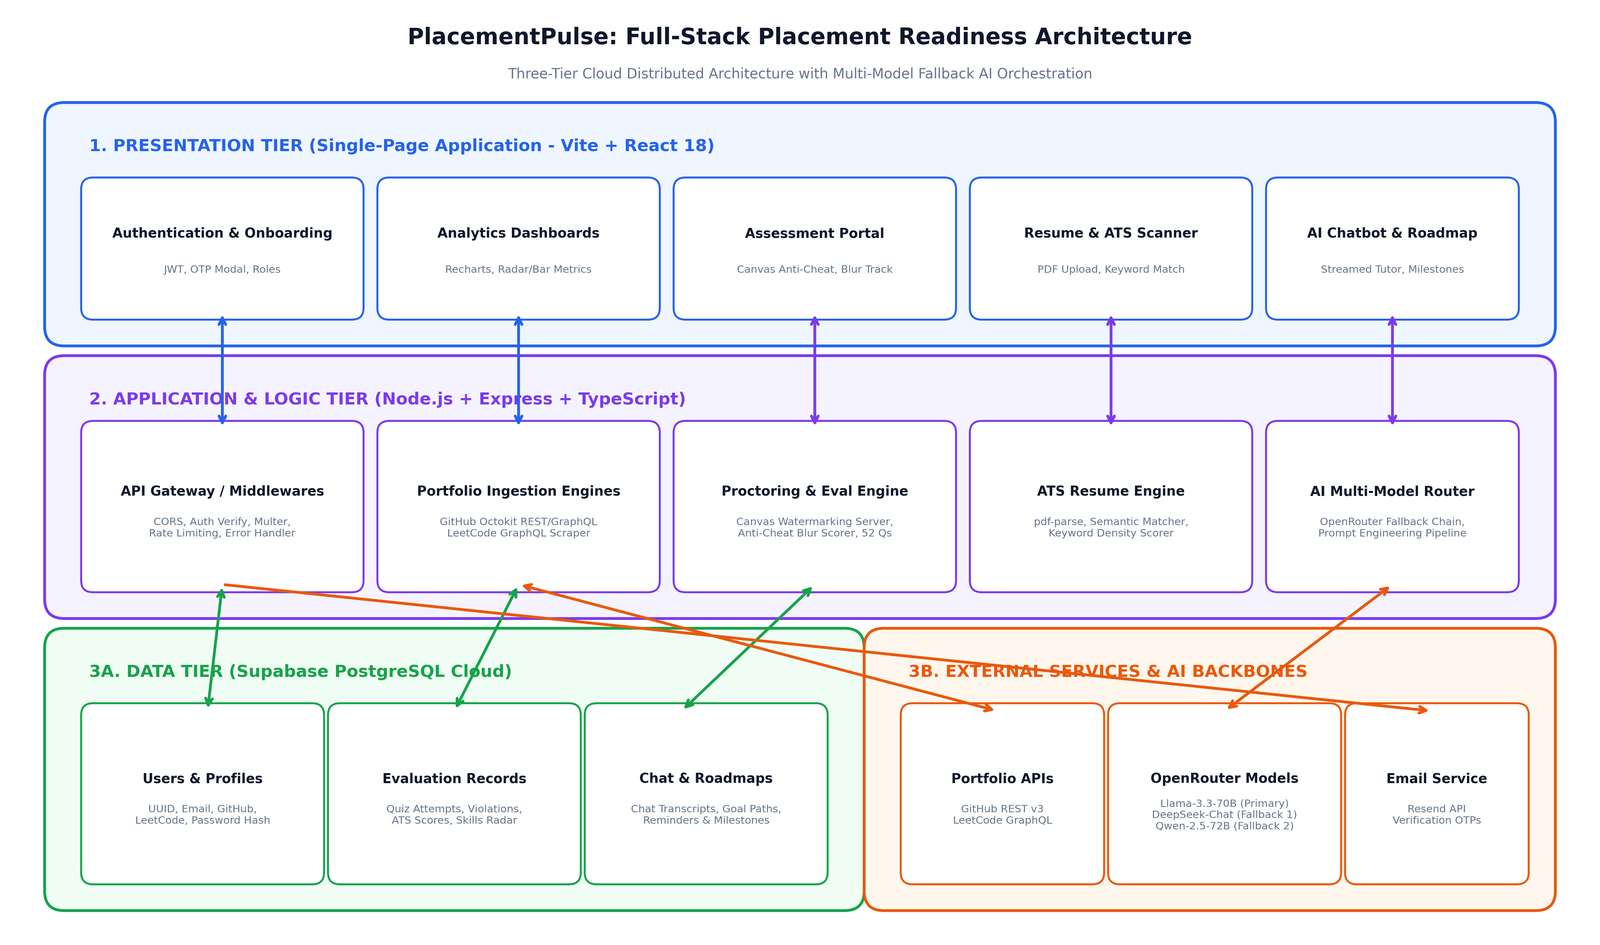
\includegraphics[width=0.85\textwidth]{figures/system_architecture.png}
\caption{PlacementPulse: End-to-End System Architecture}
\label{fig:overall_architecture}
\end{figure}

The system processes requests through a clean bidirectional execution path:
\begin{enumerate}
    \item \textbf{Presentation Tier:} A Single Page Application (SPA) built using Vite, React 18, TypeScript, and TailwindCSS that communicates with the backend over TLS 1.3 via Axios clients.
    \item \textbf{Application Logic Tier:} Express.js controllers enforcing CORS policies, JWT session authorization, Multer multipart stream buffering, and domain-specific scoring logic.
    \item \textbf{Data and AI Tier:} Managed Supabase PostgreSQL cloud instance enforcing relational integrity, alongside an OpenRouter AI gateway providing resilient multi-model LLM access.
\end{enumerate}

\section{Frontend Design}
The frontend presentation layer is structured for maximum visual fidelity, responsiveness, and minimal client-side bundle size:
\begin{itemize}
    \item \textbf{Core Stack:} React 18 and TypeScript bundled with Vite for rapid Hot Module Replacement.
    \item \textbf{Styling and Visualization:} TailwindCSS dark-mode slate theme with glassmorphic cards and Lucide-React iconography. Recharts renders dynamic multi-axis radar charts mapping competency across six core domains.
    \item \textbf{Proctored Assessment View:} Implements an HTML5 2D Canvas engine (\texttt{<canvas>}) that programmatically rasterizes examination question text, preventing browser DOM tree inspection. Window blur and document visibility listeners immediately record unauthorized tab-switching actions.
\end{itemize}

\section{Backend Design}
The backend service layer is engineered using Node.js with TypeScript in native ES Module mode:
\begin{itemize}
    \item \textbf{Routing Pipeline:} Modular Express routers handling authentication (\texttt{/api/auth}), telemetry ingestion (\texttt{/api/github}, \texttt{/api/leetcode}), in-memory ATS resume auditing (\texttt{/api/resume}), 52-question diagnostic assessments (\texttt{/api/quiz}), and conversational AI mentoring (\texttt{/api/chat}).
    \item \textbf{Security Middlewares:} Stateless JWT validation, \texttt{bcryptjs} password hashing with 10 salt rounds, and central error handling with typed response contracts.
\end{itemize}

\section{Database Design}
The persistence layer utilizes Supabase PostgreSQL. Table~\ref{tab:database_schema} summarizes the primary relational tables, column datatypes, and constraints.

\begin{table}[htbp]
\centering
\scriptsize
\caption{PlacementPulse Relational Database Schema}
\label{tab:database_schema}
\begin{tabularx}{\textwidth}{l l l X}
\toprule
\textbf{Table Name} & \textbf{Column Name} & \textbf{Data Type} & \textbf{Description / Constraints} \\
\midrule
\texttt{users} & \texttt{id} & UUID & Primary Key (\texttt{gen\_random\_uuid()}) \\
& \texttt{email} & VARCHAR(255) & Unique, Not Null \\
& \texttt{password\_hash} & VARCHAR(255) & Salted \texttt{bcrypt} hash \\
& \texttt{is\_verified} & BOOLEAN & Email OTP verification status \\
& \texttt{target\_role} & VARCHAR(100) & Desired software engineering role \\
\addlinespace
\texttt{github\_analyses} & \texttt{user\_id} & UUID & Foreign Key $\rightarrow$ \texttt{users(id)} ON DELETE CASCADE \\
& \texttt{username} & VARCHAR(100) & GitHub username handle \\
& \texttt{total\_repos} & INT & Public repository count \\
& \texttt{languages} & JSONB & Language byte share mapping \\
& \texttt{score} & NUMERIC(5,2) & Normalized GitHub hygiene score (0--100) \\
\addlinespace
\texttt{leetcode\_analyses} & \texttt{user\_id} & UUID & Foreign Key $\rightarrow$ \texttt{users(id)} ON DELETE CASCADE \\
& \texttt{username} & VARCHAR(100) & LeetCode username handle \\
& \texttt{easy/med/hard} & INT & Problem counts solved per difficulty \\
& \texttt{score} & NUMERIC(5,2) & Normalized algorithmic score (0--100) \\
\addlinespace
\texttt{resume\_analyses} & \texttt{user\_id} & UUID & Foreign Key $\rightarrow$ \texttt{users(id)} ON DELETE CASCADE \\
& \texttt{ats\_score} & NUMERIC(5,2) & Calculated ATS percentage match \\
& \texttt{matched\_skills} & TEXT[] & Array of extracted valid skills \\
\addlinespace
\texttt{quiz\_attempts} & \texttt{user\_id} & UUID & Foreign Key $\rightarrow$ \texttt{users(id)} ON DELETE CASCADE \\
& \texttt{set\_name} & VARCHAR(10) & Attempted test set (Set A, B, C) \\
& \texttt{score} & NUMERIC(5,2) & Diagnostic percentage score achieved \\
& \texttt{violations} & INT & Recorded window blur count \\
\bottomrule
\end{tabularx}
\end{table}

\section{Chatbot / AI Agent Design}
The AI mentoring assistant utilizes an autonomous multi-model fallback chain across OpenRouter. Inbound queries are routed to \texttt{Meta-Llama-3.3-70B-Instruct}. If the primary model encounters rate limits (HTTP 429) or timeouts ($>8$s), the system transparently cascades to \texttt{DeepSeek-Chat}, and subsequently to \texttt{Qwen-2.5-72B-Instruct}. A rolling context buffer retains recent conversational turns, while strict system prompts guide students conceptually without disclosing exam solutions.

\section{Data Flow / Workflow}
Figure~\ref{fig:workflow_diagram} depicts the 5-stage workflow of PlacementPulse, matching the multi-stage ingestion architecture.

\begin{figure}[htbp]
\centering
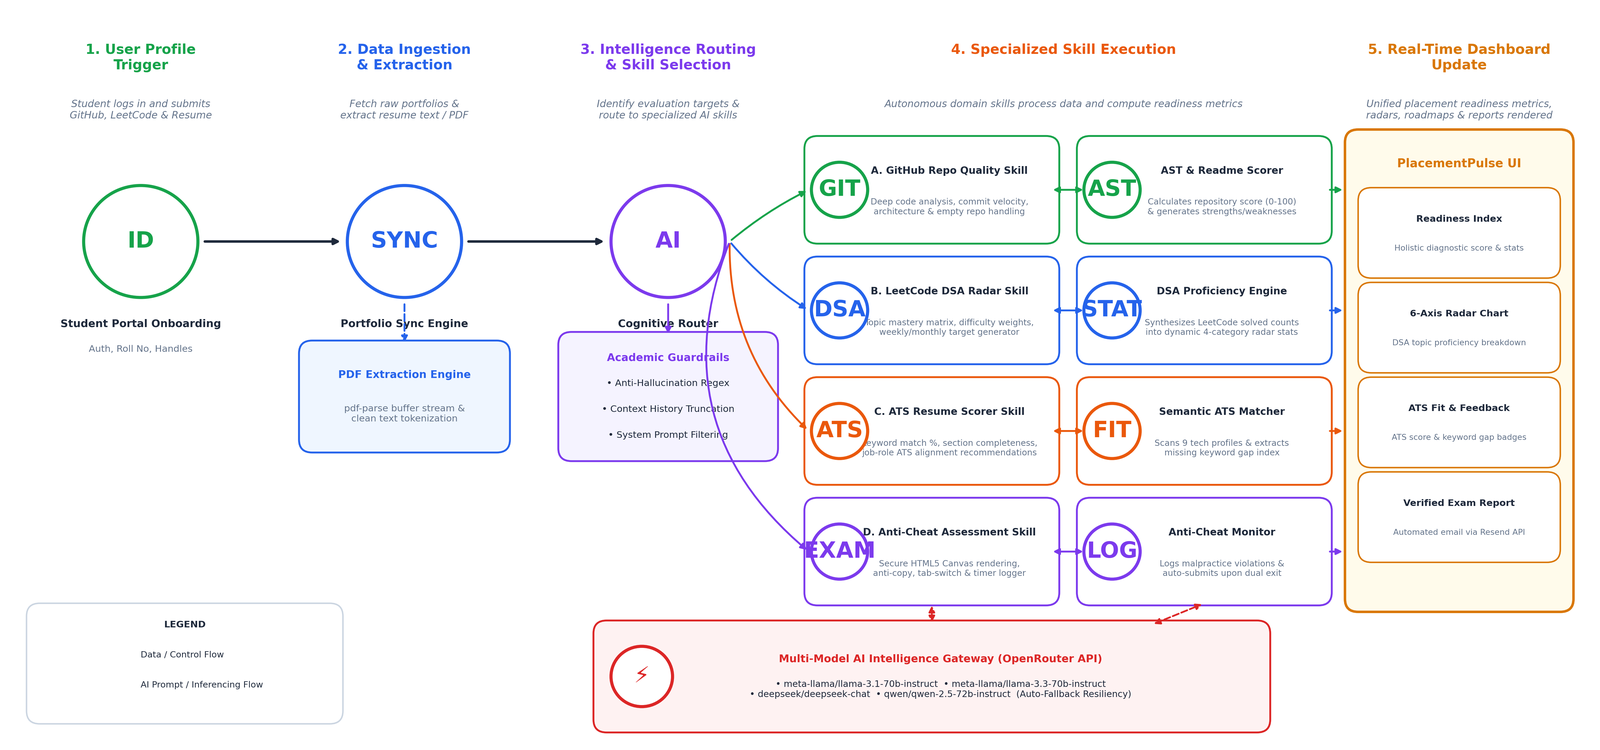
\includegraphics[width=0.88\textwidth]{figures/workflow_diagram.png}
\caption{PlacementPulse End-to-End System Workflow Diagram}
\label{fig:workflow_diagram}
\end{figure}

The workflow progresses across five stages: (1) User Profile Trigger (Registration \& Handles input); (2) Data Ingestion \& Extraction (REST/GraphQL queries and PDF parsing); (3) Intelligence Routing \& Skill Selection; (4) Specialized Skill Execution (GitHub audit, LeetCode classification, ATS screening, Canvas proctored exam); and (5) Real-Time Dashboard Update (Radar charts, Readiness Index, AI tutoring).
